\documentclass{beamer}

%\usetheme{Dresden}
\usepackage{tikz}
\usetikzlibrary{shapes}
\usepackage{grffile}
\usepackage{amsmath,empheq}

\usepackage[utf8]{inputenc}
\newcommand{\N}{\ensuremath{\mathbbm{N}}}
\newcommand{\Z}{\ensuremath{\mathbbm{Z}}}
\newcommand{\Q}{\ensuremath{\mathbbm{Q}}}
\newcommand{\R}{\ensuremath{\mathbbm{R}}}
\newcommand{\C}{\ensuremath{\mathbbm{C}}}
\renewcommand{\d}{\ensuremath{\mathrm{d}}}
\newcommand{\e}{\ensuremath{\mathrm{e}}}
\renewcommand{\L}{\ensuremath{\mathcal{L}}}
\renewcommand{\i}{\ensuremath{i}}
\newcommand{\re}{\ensuremath{\mathrm{Re}}}
\newcommand{\im}{\ensuremath{\mathrm{Im}}}
\newcommand{\At}{\ensuremath{{\phi}}}
\newcommand{\sympy}{SymPy}
%\renewcommand{\i}{\ensuremath{\mathrm{i}}}
\newcommand{\ket}[1]{|#1\rangle}
\newcommand{\bra}[1]{\langle#1|}
\newcommand{\braket}[2]{\bra{#1}#2\rangle}
\newcommand{\bracket}[3]{\bra{#1}#2\ket{#3}}

%\usepackage{units}
\usepackage{graphicx}
\usepackage{color}
\newcommand{\fig}[2]{
\begin{figure}
\centering
\includegraphics[width=10cm]{figs/#1}
\caption{#2}
\end{figure}
}





\begin{document}
\title{Holographic Methods for Condensed Matter Physics}   
\author{Petter Säterskog} 
\date{\today} 

\frame{\titlepage} 

\begin{frame}
\frametitle{Introduction}
The AdS/CFT correspondence was conjectured in 1998 by Juan Maldacena.\\

It is a correspondence between a gravitational theory and a conformal field theory.\\

It will here be used to model a high $T_c$ superconductor by a gravitational theory.\\

The application will be described and the results will be presented.\\

The work initially closely follows that of Sean Hartnoll \cite{hartnoll8}.
\end{frame}

\begin{frame}
\frametitle{Outline}
\begin{itemize}
  \item What is AdS?
  \item The AdS/CFT correspondence
  \item High $T_c$ superconductors
  \item Application of the correspondence
  \item Results: condensate developement, conductivity
  \item Extended model
  \item Results: conductivity, fit of Drude model
  \item Conclusion
  \end{itemize}
\end{frame}

\begin{frame}
\frametitle{Anti de Sitter space (AdS)}
Einsteins equation with negative cosmological constant $\Lambda$
\begin{equation}
R_{ab}-\frac{1}{2}g_{ab}R+g_{ab}\Lambda=\kappa T_{ab}\label{einstein}
\end{equation}
has AdS as solution, just like $\Lambda=0$ gives flat space.
\begin{equation}
 g_{ab}\d x^a\d x^b=\frac{L^2}{z^2}\left(-\d t^2+\d x^2+\d y^2+\d z^2\right).\label{metric}
\end{equation}
\end{frame}

\begin{frame}
\frametitle{The AdS/CFT correspondence}
Gravitational theory in AdS space / Conformal field theory
\begin{equation}
 Z_{\mathrm{bulk}}(\delta\psi_{(0)})=\left\langle\exp(\i\int\d^dx\sqrt{g_0}\delta\psi_{(0)}\mathcal{O})\right\rangle_{\mathrm{CFT}}\label{fulCorr}
\end{equation}
\end{frame}

\begin{frame}
\frametitle{Overview}
\begin{figure}
 \centering
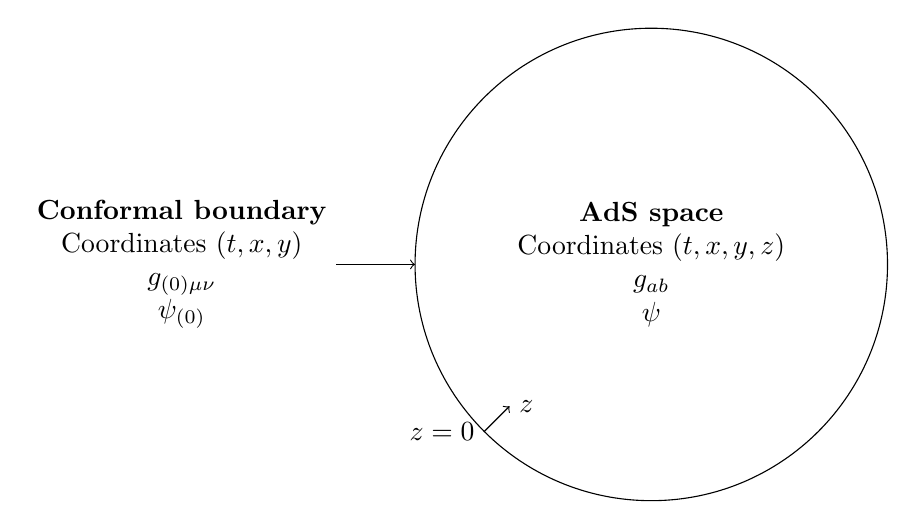
\begin{tikzpicture}
\draw (0,0) circle (3cm) node[align=center] {{\bf AdS space}\\Coordinates $(t,x,y,z)$\\$g_{ab}$\\$\psi$};
\draw[<-] (-3,0) -- (-4,0) node[left,align=center] {{\bf Conformal boundary}\\Coordinates $(t,x,y)$\\$g_{(0)\mu\nu}$\\$\psi_{(0)}$};
\draw[->] ({-3/sqrt(2)},{-3/sqrt(2)}) -- (-1.8,-1.8) node[right,align=center] {$z$};
\draw ({-3/sqrt(2)},{-3/sqrt(2)})  node[left,align=center] {$z=0$};
\end{tikzpicture}
\end{figure}
\end{frame}

\begin{frame}
\frametitle{Classical approximation}
Boundary gauge theory with many colors, large $N$.\\
$\implies$\\
Classical bulk theory.\\
\vspace{0.5cm}
We do not even have an $N$. A similar effect is expected for certain strongly coupled gauge theories. See e.g. \emph{Holographic duality with a view toward many-body physics} by John McGreevy for a motivation of why we can assume a classical bulk.\\
\vspace{0.5cm}
This is a major headache for AdS/CFT, the bulk theory should be a stringy quantum gravity theory without the large $N$ and not very useful.\\
\vspace{0.5cm}
The strength of the AdS/CFT approach to condensed matter physics comes from that we can do otherwise intractable calculations on strongly coupled systems.
\end{frame}

%oldframes


\begin{frame}
\frametitle{Temperature}
Field theory expectation values at a finite temperature are calculated using a Euclidean path integral with periodic time.\\
This corresponds to a metric periodic in Euclidean time on the AdS side of the correspondence.\\
The solution to the Einstein equation satisfying this boundary condition is a black hole in AdS space.
\end{frame}

\begin{frame}
\frametitle{Black Hole}
\begin{figure}
 \centering
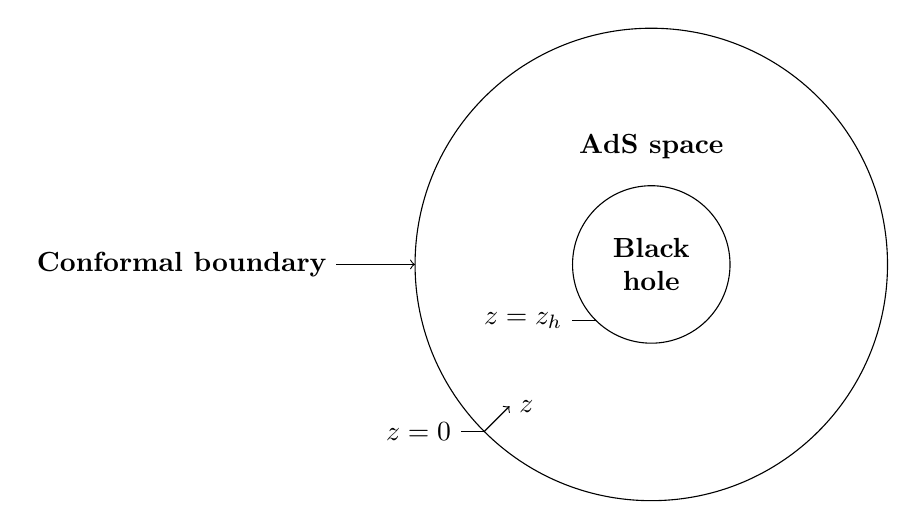
\begin{tikzpicture}
\draw (0,1.5)  node[align=center] {{\bf AdS space}};
\draw (0,0) circle (3cm) node[align=center] {{\bf Black}\\{\bf hole}};
\draw (0,0) circle (1cm);
\draw[<-] (-3,0) -- (-4,0) node[left,align=center] {{\bf Conformal boundary}};
\draw[->] ({-3/sqrt(2)},{-3/sqrt(2)}) -- (-1.8,-1.8) node[right,align=center] {$z$};
\draw[-] ({-3/sqrt(2)},{-3/sqrt(2)}) -- ({-3/sqrt(2)-0.3},{-3/sqrt(2)})  node[left,align=center] {$z=0$};
\draw[-] ({-1/sqrt(2)},{-1/sqrt(2)}) -- ({-1/sqrt(2)-0.3},{-1/sqrt(2)})  node[left,align=center] {$z=z_h$};
\end{tikzpicture}
\end{figure}
\end{frame}


\begin{frame}
\frametitle{High $T_c$ Superconductors}
Much higher $T_c$ ($>$130K) than what is allowed by BCS theory ($\approx$ 30K).\\
No satisfying explanation of the phenomenon yet, possibly due to strong coupling preventing a perturbative description and numerical simulations.\\
Strongly coupled systems can be modeled by AdS/CFT.\\
\vspace{0.3cm}
Two-dimensional layered materials.\\
Effect not expected to depend on lattice vibrations, pure electromagnetic phenomenon?\\
Superconductivity possibly occurs near quantum critical point and thus exhibits scale invariance.\\
Breaking of U(1) gauge symmetry as in BCS case.
\end{frame}

\begin{frame}
\frametitle{Formulating the AdS Theory Corresponding to a High $T_c$ Superconductor}
$\psi_{0}$ - Scalar field appearing below $T_c$.\\
$A_{0a}$ - Electromagnetic potential.\\
No phonons, no lattice, no spatial variation, no magnetic field.\\
\vspace{1cm}
\begin{tabular}{ r | l }
CFT & AdS \\
1+2 dimensions & 1+3 dimensions\\
temperature $T$ & horizon at $z_h=\frac{3}{4\pi T}$ \\
$\mathcal{O}$, $\psi_{0}$&$\psi(z)$\\
$J_a$, $A_{a,(0)}$&$A(t,z)$\\
{\bf Strongly coupled quantum theory} & {\bf Classical theory}
\end{tabular}
\end{frame}

\begin{frame}
\frametitle{Overview}
\begin{figure}
 \centering
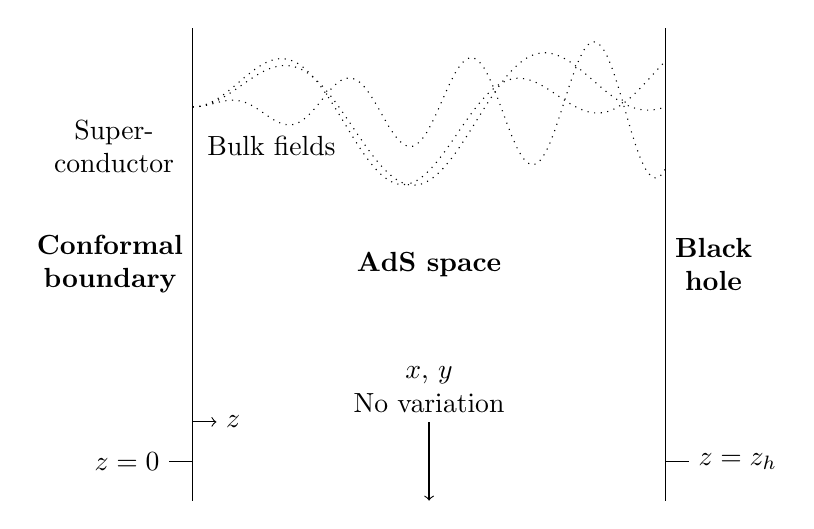
\begin{tikzpicture}
\draw (0,0) -- (0,6);
\draw (0,3) node[left,align=center] {{\bf Conformal}\\{\bf boundary}};
\draw (6,0) -- (6,6);
\draw (6,3) node[right,align=center] {{\bf Black}\\{\bf hole}};
\draw (3,3) node[align=center] {{\bf AdS space}};
\draw[->] (0,1) -- (0.3,1) node[right,align=center] {$z$};
\draw[-]  (0,0.5)--(-0.3,0.5)  node[left,align=center] {$z=0$};
\draw[-]  (6,0.5)--(6.3,0.5)  node[right,align=center] {$z=z_h$};
\draw[<-] (3,0) -- (3,1) node[above,align=center] {$x$, $y$\\No variation};
\draw[dotted] plot[domain=0:6,samples=100] (\x,{sin(\x *100.)*sin(\x *37.)+5});
\draw[dotted] plot[domain=0:6,samples=100] (\x,{sin(\x *30.)*sin(\x *97.)+5});
\draw[dotted] plot[domain=0:6,samples=100] (\x,{sin(\x *230.)*sin(\x *11.)+5});
\draw[-] (1,4.5) node[align=center] {Bulk fields};
\draw[-] (-1,4.5) node[align=center] {Super-\\conductor};
\end{tikzpicture}
\end{figure}
\end{frame}

\begin{frame}
\frametitle{Bulk Theory}
A bulk theory Lagrangian of the following form has been used.
\begin{eqnarray}
 \mathcal{L}=&\frac{1}{2\kappa}\left(R-2\Lambda\right)-\frac{1}{4}F_{ab}F^{ab}-m^2|\psi|^2-|D_a\psi|^2
\label{L}
\end{eqnarray}
Includes the lowest order terms obeying symmetry requirements. A higher order term will later be included.
\end{frame}

\begin{frame}
\frametitle{Equations of Motion}
The equations of motion are obtained by varying the Lagrangian with respect to the different fields,
\begin{equation}
\begin{split}
\left(m^2-\nabla^2+q^2A^2+\i q(\nabla_aA^a)\right)\psi&=0\\
 -\nabla_aF^{ab}+2q^2|\psi|^2A^b+iq\left(\overline{\psi}\nabla^b\psi-\psi\nabla^b\overline{\psi}\right)&=0.
 \end{split}
\end{equation}
After using the metric, translational invariance, harmonic time-dependence, infinitesimal $A_x$, and making a choice of gauge we have
\begin{empheq}[left=\empheqlbrace]{align}
   &\Big(q^2z^2\phi^2-L^2m^2f+zf(zf^\prime-2f)\partial_z+z^2f^2\partial_z\partial_z\Big)\psi=0\\
 &\Big(-2q^2\psi^2L^2+z^2f\partial_z\partial_z\Big)\phi=0\\
 &\Big(-2q^2\psi^2L^2f+z^2\omega^2+z^2ff^\prime\partial_z+z^2f^2\partial_z\partial_z\Big)A_x=0.
\end{empheq}
This is a system of non-linear ordinary differential equations.
\end{frame}

\begin{frame}
\frametitle{Solving Ordinary Differential Equations}
There is a trivial solution to the equations
\begin{empheq}[left=\empheqlbrace]{align}
 &\psi(z)=0 \nonumber\\
 &\phi(z)=\mu(1-z/z_h) \nonumber\\
 &A_x(z)=
\left[
\exp\left( - \sqrt{3}\tan^{-1} \frac{z_h+2z}{z_h\sqrt{3}} \right)
\frac{z_h-z}{\sqrt{z^2+zz_h+z_h^2}}
\right]^{\frac{\i\omega z_h}{3} }   \label{trivial} \nonumber
\end{empheq}
Finding an analytical solution with $\psi\neq0$ is hard so a numerical integrator has been used for this.
\end{frame}


\begin{frame}
\frametitle{Results of Scalar Operator}
\begin{figure}
\centering
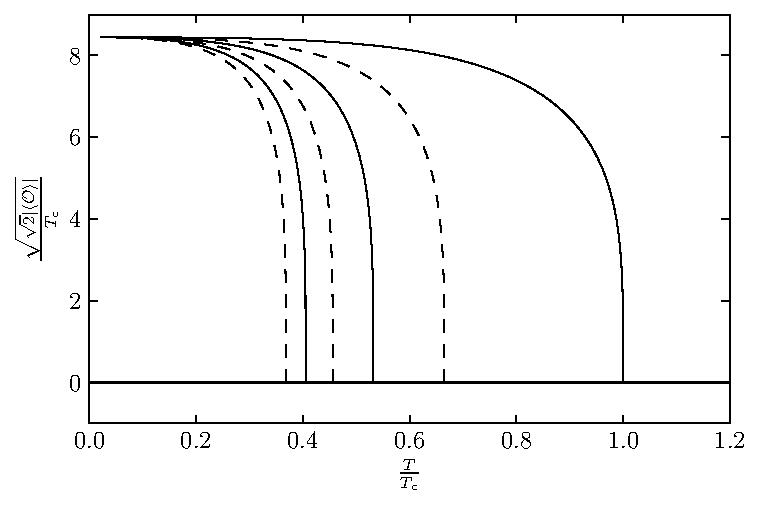
\includegraphics[width=8cm]{figs/O_constRho_a2_0.0.pdf}
\caption{Expectation value of CFT operator $\mathcal{O}$ at different $T$ and constant $\rho$. The multiple curves correspond to multiple solutions at the same temperature. The dashed lines have different signs of the expectation value of $\mathcal{O}$ and the horizon boundary condition $\psi(z_h)$. Further solutions (here ommited) are obtained for lower temperature following the trend shown here.}
\end{figure}
\end{frame}


\begin{frame}
\frametitle{Results of Conductivity}
\fig{cond_Ts_a2_0.0_v2.pdf}{Real and imaginary part of the conductivity for different temperatures. $\rho$ is here constant.\label{f:cond}}
%$\delta$-function at $\omega=0$
%The Kramers-Kronig relation relates the real and imaginary part of response functions of causal systems. This can be used to show that there is a $\delta$-function in the conductivity at $\omega=0$.
\end{frame}

\begin{frame}
\frametitle{Sum Rule}

\begin{figure}
\centering
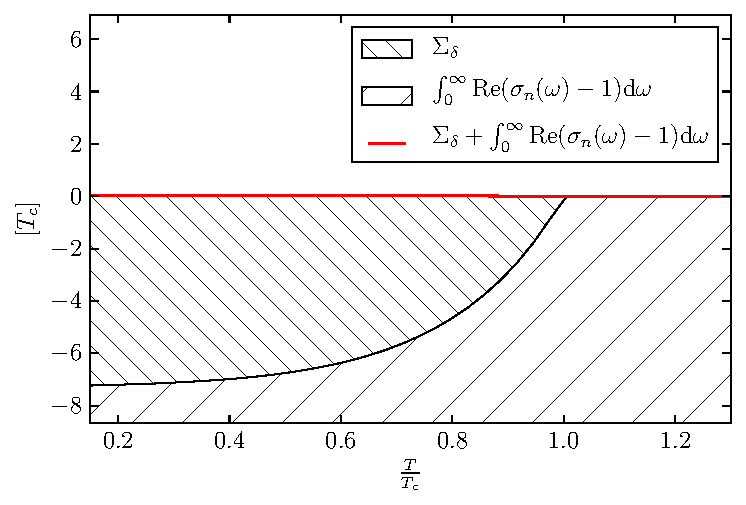
\includegraphics[width=7.5cm]{figs/sum_rule_a20}
\caption{The two contributions to the integral in the modified Ferrell-Glover-Tinkham sum rule for different temperatures. The red line is expected to be precisely at 0 for perfect numerics}
\end{figure}
\end{frame}



\begin{frame}
\frametitle{Comparison with Experiments on Graphene}
\begin{columns}
\begin{column}{6cm}
\begin{figure}
\centering
\includegraphics[width=5cm]{figs/stolen.png}
\end{figure}
\end{column}
\begin{column}{6cm}
\begin{figure}
\centering
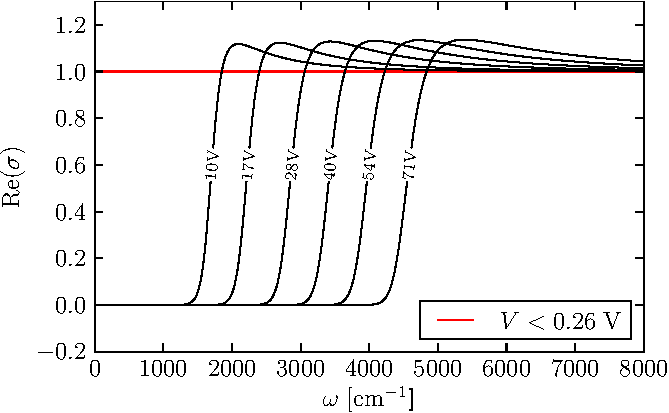
\includegraphics[width=5cm]{figs/graphene2_cond_re_a2_0.0-crop.pdf}\\
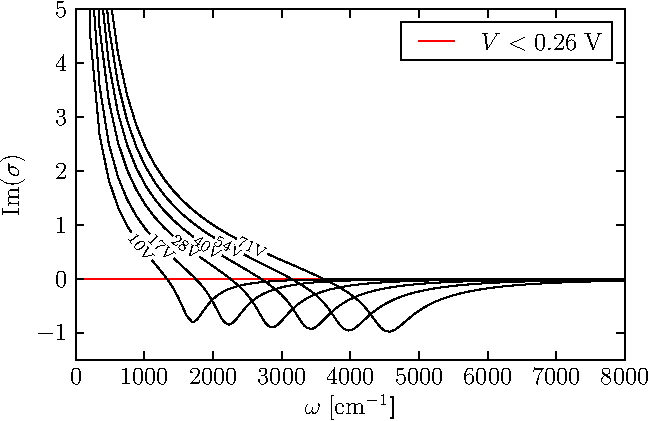
\includegraphics[width=5cm]{figs/graphene2_cond_im_a2_0.0-crop.pdf}\\
\end{figure}
\end{column}
\end{columns}
\footnote{Image stolen from \emph{Dirac charge dynamics in graphene by infrared spectroscopy}, Li et al.~,Nature Physics}
\end{frame}

\begin{frame}
\frametitle{Drude model}
The charge carriers are assumed to obey the equation of motion
\begin{equation}
 \frac{\d v}{\d t}=\frac{q}{m}E-\frac{1}{\tau}v.
\end{equation}
This gives the conductivity
\begin{equation}
  \sigma(\omega)=\frac{J(\omega)}{E(\omega)}=\frac{\sigma_0}{1-\i\tau\omega}.
\end{equation}
\end{frame}

\begin{frame}
\frametitle{Motivating Extension to Lagrangian}
Horowitz et al.~\cite{horowitz} have studied the same Lagrangian but with a varying background electrical potential to model a periodic lattice.\\
\vspace{1cm }
They obtained a Drude peak for low frequencies.
\end{frame}

\begin{frame}
\frametitle{Extended Lagrangian}
Myers et al.~\cite{Myers:2010pk} have studied what higher order corrections of $F$ could be added to the Lagrangian.\\
These were previously studied by Tobias Wenger, Chalmers University of Technology.
One induced what looked like a Drude peak at low frequencies.
\begin{equation}
 \mathcal{L}_\mathrm{ext}=\mathcal{L}+\alpha_2F^a_{\ b}F^b_{\ c}F^c_{\ d}F^d_{\ a}
\end{equation}
\end{frame}

\begin{frame}
\fig{cond_Ts_a2_0.01_v2.pdf}{Real part of the conductivity for different temperatures using the extended Lagrangian with $\alpha_2=0.01L^4$. $\rho$ is here constant.\label{f:cond_a2_1}}
\end{frame}

\begin{frame}
\fig{cond_Ts_a2_0.1_v2.pdf}{Real part of the conductivity for different temperatures using the extended Lagrangian with $\alpha_2=0.1L^4$. $\rho$ is here constant.\label{f:cond_a2_2}}
\end{frame}

\begin{frame}
\fig{drude_T_1Tc_a2_0.1}{Conductivity for $\alpha_2=0.1L^4$ and $T=T_c$ together with Drude model fit.\label{f:drude}}
\end{frame}

\begin{frame}
\fig{drude_T_1Tc_a2_10}{Conductivity for $\alpha_2=10L^4$ and $T=T_c$ together with Drude model fit.\label{f:drude2}}
\end{frame}

\begin{frame}
\fig{drudeVara2_T=2Tc}{Drude parameters as functions of $\alpha_2$ at $T=2T_c$.\label{f:drudeVar}}
\end{frame}

\begin{frame}
\fig{drudeVarMT}{$\omega\rightarrow0$ limit of the conductivity as a function of $\alpha_2$ for different temperatures.\label{f:drudeVarT}}
\end{frame}

\begin{frame}
\fig{drudeTdep_1e4}{$\sigma_0L^4/\alpha_2$ as a function of temperature for large $\alpha_2$.\label{f:Cdep}}
\end{frame}

\begin{frame}
This analysis gives the asymptotic behaviour of the DC-conductivity
\begin{equation}
 \sigma_0=C\frac{\alpha_2}{L^4}\left(\frac{T}{T_c}\right)^{-4/3}.
\end{equation}
This gives a $T^{4/3}$ dependence on the scattering rate $1/\tau$, whereas a $T^1$ dependence is observed experimentally for the cuprates \cite{drudeFit}.\\

Our way of obtaining the Drude peak is computationally much simpler than the periodic lattice and might be a useful effective description.\\
\end{frame}

\begin{frame}
\frametitle{Summary}
\begin{itemize}
\item We have modeled a high $T_c$ superconductor using the AdS/CFT correspondence.
\item An scalar field coupled to an electromagnetic field has been used.
\item A superconducting phase and conductance gap is shown to appear below $T_c$.
\item The conductivity sum rule is satisfied indicating correct and accurate calculations.
\item An addition is made to the Lagrangian giving a peak in the conductivity.
\item The extended Lagrangian gives a conductivity closer to experiments above $T_c$ since we have a conductivity peak around $\omega=0$.
\item The Drude model gives a surprisingly accurate fit to this peak.
\end{itemize}
\end{frame}

\begin{frame}
\frametitle{Outlook}
\begin{itemize}
\item Compare with Horowitz et al.~$T$-dependence.
\item Compare with experiments below $T_c$.
\item Understand graphene model.
\item Understand ODEs better.
\end{itemize}
\end{frame}

\begin{frame}
\bibliographystyle{unsrt}
\bibliography{report}
\end{frame}

\begin{frame}
\frametitle{Questions? (Please not too hard\footnote{large N...})}
\end{frame}

\begin{frame}
\frametitle{The AdS/CFT correspondence}
Gravitational theory in AdS space / Conformal field theory
\begin{equation}
 Z_{\mathrm{bulk}}(\delta\psi_{(0)})=\left\langle\exp(\i\int\d^dx\sqrt{g_0}\delta\psi_{(0)}\mathcal{O})\right\rangle_{\mathrm{CFT}}\label{fulCorr}
\end{equation}
The equations of motion in the bulk give the following boundary behaviour
\begin{equation}
 \psi(z)=\left(\frac{z}{L}\right)^{\Delta_{(0)}}\psi_{(0)}+
\left(\frac{z}{L}\right)^{\Delta_{(1)}}\psi_{(1)}+...
\end{equation}
\end{frame}

\begin{frame}
\frametitle{CFT operators}
Background fields in the CFT are sources to operators
\begin{equation}
\mathcal{O}= \frac{\delta S_{\mathrm{CFT}}}{\delta \psi_{(0)}}
\end{equation}
Expectation values of these can be calculated as
\begin{equation}
\begin{split}
&-\i\frac{\delta\log Z_{\mathrm{bulk}}(\psi_{(0)})}{\delta\psi_{(0)}(x)}|_{\psi_{(0)}=0}\\
&=-\i\frac{\delta\log\left\langle\exp(\i\int\d^dx\sqrt{g_{(0)}}\psi_{(0)}\mathcal{O})\right\rangle_{\mathrm{CFT}}}{\delta\psi_{(0)}(x)}|_{\psi_{(0)}=0}\\
&=\frac{\left\langle\mathcal{O}(x)\exp(\i\int\d^dx\sqrt{g_{(0)}}\psi_{(0)}\mathcal{O})\right\rangle_{\mathrm{CFT}}}{\left\langle\exp(\i\int\d^dx\sqrt{g_{(0)}}\psi_{(0)}\mathcal{O})\right\rangle_{\mathrm{CFT}}}|_{\psi_{(0)}=0}\\
&=\langle \mathcal{O}(x) \rangle_{\mathrm{CFT}}
\end{split}
\end{equation}
\end{frame}




\begin{frame}
\frametitle{Classical Approximation for Obtaining Expectation Values}
The way to calculate expectation values shown earlier needed the bulk partition function.\\
This can be obtained in a classical limit as
\begin{equation}
 Z_{\mathrm{bulk}}(\psi_{(0)})=C\exp(\i S_c)\label{semi}
\end{equation}
$S_c$ is the saddle point action of the Lagrangian. We then have 
\begin{equation}
\langle \mathcal{O}(x) \rangle_{\mathrm{CFT}}=\frac{\delta S_c(\psi_{(0)})}{\delta\psi_{(0)}(x)}|_{\psi_{(0)}=0}
\end{equation}
This lets us calculate CFT expectation values by solving the bulk equations of motion.
\end{frame}


\begin{frame}
\frametitle{Expectation Values from Boundary Behaviour of Bulk Fields}
Using the equations of motion and boundary behaviour of fields one arrives at
\begin{equation}
\langle \mathcal{O}(x) \rangle_{\mathrm{CFT}}=\frac{\delta S_c(\psi_{(0)})}{\delta\psi_{(0)}(x)}|_{\psi_{(0)}=0}
=\frac{2\psi_{(1)}}{L}
\end{equation}
Suitable boundary terms to the Lagrangian must be considered for arriving at this expression. Read my report for more details :).\\
Similar expressions can be obtained for tensor fields, e.g.\\
 \begin{equation}
 \langle J_a\rangle_{\mathrm{CFT}}=\frac{A_{a(1)}}{L}
\end{equation}
\end{frame}


\end{document}

